%%
%% This is file `sample-manuscript.tex',
%% generated with the docstrip utility.
%%
%% The original source files were:
%%
%% samples.dtx  (with options: `manuscript')
%% 
%% IMPORTANT NOTICE:
%% 
%% For the copyright see the source file.
%% 
%% Any modified versions of this file must be renamed
%% with new filenames distinct from sample-manuscript.tex.
%% 
%% For distribution of the original source see the terms
%% for copying and modification in the file samples.dtx.
%% 
%% This generated file may be distributed as long as the
%% original source files, as listed above, are part of the
%% same distribution. (The sources need not necessarily be
%% in the same archive or directory.)
%%
%% The first command in your LaTeX source must be the \documentclass command.
\documentclass[manuscript,screen]{acmart}
\usepackage{graphicx}
\graphicspath{ {./images/} }
\usepackage{fancyvrb}
\usepackage{multirow}
\usepackage[section]{placeins}
%%
%% \BibTeX command to typeset BibTeX logo in the docs
\AtBeginDocument{%
  \providecommand\BibTeX{{%
    \normalfont B\kern-0.5em{\scshape i\kern-0.25em b}\kern-0.8em\TeX}}}

%% Rights management information.  This information is sent to you
%% when you complete the rights form.  These commands have SAMPLE
%% values in them; it is your responsibility as an author to replace
%% the commands and values with those provided to you when you
%% complete the rights form.
\setcopyright{acmcopyright}
\copyrightyear{2022}
\acmYear{2022}
%\acmDOI{10.1145/1122445.1122456}

%% These commands are for a PROCEEDINGS abstract or paper.
\acmConference [RecSys'22] 
{Seattle, WA USA}
{16th ACM Conference on Recommender Systems, Seattle, WA USA, Sept. 18 - 23, 2022}

\acmBooktitle{16th ACM Conference on Recommender Systems,  Seattle, WA USA, Sept. 18 - 23, 2022}

\acmPrice{15.00}
\acmISBN{978-1-4503-XXXX-X/18/06}


%%
%% Submission ID.
%% Use this when submitting an article to a sponsored event. You'll
%% receive a unique submission ID from the organizers
%% of the event, and this ID should be used as the parameter to this command.
%%\acmSubmissionID{123-A56-BU3}

%%
%% The majority of ACM publications use numbered citations and
%% references.  The command \citestyle{authoryear} switches to the
%% "author year" style.
%%
%% If you are preparing content for an event
%% sponsored by ACM SIGGRAPH, you must use the "author year" style of
%% citations and references.
%% Uncommenting
%% the next command will enable that style.
%%\citestyle{acmauthoryear}

%%
%% end of the preamble, start of the body of the document source.
\begin{document}

%%
%% The "title" command has an optional parameter,
%% allowing the author to define a "short title" to be used in page headers.
\title{Impact of Variations of Similarity and Prediction Techniques on User-based and Item-based Collaborative Filtering Recommendations}

%%
%% The "author" command and its associated commands are used to define
%% the authors and their affiliations.
%% Of note is the shared affiliation of the first two authors, and the
%% "authornote" and "authornotemark" commands
%% used to denote shared contribution to the research.

\author{Anh Hoang}
\affiliation{%
  \institution{Davidson College}
  \streetaddress{102 N Main Street}
  \city{ Davidson}
  \state{ North Carolina}
  \postcode{ 28035}
  \country{USA} }
\email{duhoang@davidson.edu}

\author{Mengfan Wang}
\affiliation{%
  \institution{Davidson College}
  \streetaddress{102 N Main Street}
  \city{ Davidson}
  \state{ North Carolina}
  \postcode{ 28035}
    \country{USA} } 
\email{mewang@davidson.edu}

\author{Mike Remezo}
\affiliation{%
  \institution{Davidson College}
  \streetaddress{102 N Main Street}
  \city{ Davidson}
  \state{ North Carolina}
  \postcode{ 28035}
    \country{USA} } 
\email{miremezo@davidson.edu}

\author{Malavika Kalani}
\affiliation{%
  \institution{Davidson College}
  \streetaddress{102 N Main Street}
  \city{ Davidson}
  \state{ North Carolina}
  \postcode{ 28035}
    \country{USA} } 
\email{makalani@davidson.edu}

%%
%% By default, the full list of authors will be used in the page
%% headers. Often, this list is too long, and will overlap
%% other information printed in the page headers. This command allows
%% the author to define a more concise list
%% of authors' names for this purpose.
\renewcommand{\shortauthors}{NAMES: Anh Hoang, Mengfan Wang, Mike Remezo, Malavika Kalani}

%%
%% The abstract is a short summary of the work to be presented in the
%% article.
\begin{abstract}
Given a wide array of implementations of recommender systems that were developed as a result of the exponential growth of the recommender system-related research field, it is of great importance to be able to measure these different algorithms against each other and perform an objective analysis of their functionality. In this paper, we dismantle the two most popular recommender methods, collaborative filtering and content-based methods, into separate components to evaluate each of them when accompanied by different similarity and prediction parameters. We seek to propose the best prediction algorithm - one that we define to be the recommending implementation that demonstrates the highest level of accuracy and coverage across all algorithms analyzed.
\end{abstract}

%%
%% The code below is generated by the tool at http://dl.acm.org/ccs.cfm.
%% Please copy and paste the code instead of the example below.
%%
%\begin{CCSXML}
%<ccs2012>
% <concept>
%  <concept_id>10010520.10010553.10010562</concept_id>
%  <concept_desc>Computer systems organization~Embedded systems</concept_desc>
%  <concept_significance>500</concept_significance>
% </concept>
% <concept>
%  <concept_id>10010520.10010575.10010755</concept_id>
%  <concept_desc>Computer systems organization~Redundancy</concept_desc>
%  <concept_significance>300</concept_significance>
% </concept>
% <concept>
%  <concept_id>10010520.10010553.10010554</concept_id>
%  <concept_desc>Computer systems organization~Robotics</concept_desc>
%  <concept_significance>100</concept_significance>
% </concept>
% <concept>
%  <concept_id>10003033.10003083.10003095</concept_id>
%  <concept_desc>Networks~Network reliability</concept_desc>
%  <concept_significance>100</concept_significance>
% </concept>
%</ccs2012>
%\end{CCSXML}
%
%\ccsdesc[500]{Computer systems organization~Embedded systems}
%\ccsdesc[300]{Computer systems organization~Redundancy}
%\ccsdesc{Computer systems organization~Robotics}
%\ccsdesc[100]{Networks~Network reliability}

%%
%% Keywords. The author(s) should pick words that accurately describe
%% the work being presented. Separate the keywords with commas.
\keywords{Recommender Systems, Collaborative Filtering, Similarity and Prediction techniques}


%%
%% This command processes the author and affiliation and title
%% information and builds the first part of the formatted document.
\maketitle

\section{Introduction}

%%Introduce your work effort here. Explain the motivation for undertaking this work and the importance to the Recommender System field. Include a brief discussion of research questions to be pursued/answered in this study. Indicate any novel approaches.

\hspace{\parindent}Owing to the booming growth of e-commerce in the last decade, there has been a drastic movement from the physical to virtual space with regards to consumers’ habits. Digital platforms such as Netflix and Amazon to name a few, have become an integral part of every individual's life as these platforms guarantee leisure, convenience, and efficiency. They are able to give their users a more personalized experience because of a strong network of algorithms known as \emph{Recommender Systems}, which solve the problem of how to filter, prioritize, and efficiently deliver suggestions on items that best fit consumers’ needs. 
    
    
There has been extensive research into the field of recommender systems with substantial focus placed on its two major paradigms: collaborative filtering and content-based methods. Collaborative filtering generates recommendations for a user through a systematic analysis of data collected from other users sharing similar tastes or information needs. Through the use of this recommender method, the recommending process can be conducted on certain types of items that may prove to be hard to analyze with computers such as feelings, ideas, and movies. In addition, collaborative filtering allows for serendipitous recommendations, which means that it may provide users with suggestions on items beyond their expectations. Collaborative filtering also improves the quality of its recommendations as more interactions are recorded over time. On the other hand, content-based methods examine items similar to other items that a user has liked in the past. This recommender method compensates for collaborative filtering’s cold start problem, which means that the user-based algorithm requires a certain amount of data for it to work effectively; however, content-based methods don’t show potential for increasing effectiveness over time since they can only operate on users’ existing interest. Overall, both methods still present imperfections in their mechanisms; this particular problem has created an intellectual venue for a vast amount of research literature that looks into different ways of implementing a recommender system.
    
In light of the overwhelming number of existing recommender algorithms, this particular problem warrants critical analysis of these different implementations. The core recommending algorithm can be broken down into three steps for both user-based and item-based methods: (1) Apply different weightings to all users/ items to calculate the similarity among users and items (2) Create a subset of users/items to predict the ratings for an item that the user has not rated (3) Perform normalization of ratings and calculate the prediction using a weighted array of selected neighbors’ ratings\cite{her99}. During each step in the process, we can apply different similarity and prediction parameters, such as Pearson correlation and Euclidean distance for the similarity weighting, or we can choose to apply significance weighting to account for only items or users that have a very high similarity score. Given that each implementation will output different results with varying accuracy and coverage, the question of what combinations of similarity and prediction techniques will produce the best results is worthy of discussion.
    
Our paper presents an algorithmic evaluation of content-based and user-based recommender systems through different implementations of the core algorithm, which allows for fine-grained control over distinct variations of similarity and prediction parameters. Ultimately, our goal is to propose the best recommendation algorithm based on two metrics: accuracy and coverage. 


\section{Related Work}
%%This section presents the prior work that has been conducted in this area of research. Use citations and the accomplishments of the prior work.
\hspace{\parindent} In this section, we briefly present some of the research literature related to the early implementations of collaborative filtering systems as well as works related to the functioning of user and item-based recommendations. 
\newline
Recommender systems have become a popular system that most companies and platforms rely on for offering the best recommendations to users through content-based and collaborative filtering methods. Since its initial development, collaborative filtering methods  have offered more advantages than content-based filtering methods as stated by \cite{her99}. Collaborative filtering filters items based on quality and user preferences and also provides serendipitous recommendations to users as suggested by \cite{her99} in his paper \emph{An Algorithmic Framework for Performing Collaborative Filtering}. 
\newline
GroupLens, a distributed system for using ratings from other users to predict an active user’s ratings in articles, was the first to introduce an automated collaborative filtering system. GroupLens mainly used the ratings to determine which users’ ratings were most similar to each other and it used ratings from similar users to predict how well a user would like a certain article. Better Bit Bureaus (one of the entities in GroupLens’ netnews system) are servers that are used to predict ratings. In a user-based collaborative filtering system, we can calculate a predicted rating of an item not rated by a user by finding other users similar to that user who has rated that item. In a similar manner, \emph{Better Bit Bureaus} uses the opinions of other people who have already rated the articles and combines those ratings to generate a predicted rating. 
\newline
The tremendous advancement in the use of technology has led to an increase in the number of users on websites and digital platforms. The research paper \cite{bad} describes how item-based collaborative filtering systems can enable recommender systems to function at a larger scale by using the correlation between different items to make recommendations for the user. In our paper, we have shown the use of the Pearson correlation and the Euclidian distance method to compute the similarity between two items. A few research studies have also focused on other methods to compute the similarity between two items. \cite{bad} describes two other methods: cosine-based similarity (considers two items as vectors and computes the similarity by finding the cosine of the angle between them) and adjusted cosine similarity (takes into account the difference in rating scale between different users by subtracting the respective user average from each co-rated pair). 
\cite{her99} lays a strong foundation for our research as it provides a similar analysis of different algorithms to identify the most accurate recommender system. Herlocker’s detailed explanation of each component of the collaborative filtering process proves to be an integral driving force behind our findings.   
 

\section{Thesis}
%%This section explains the research that will be performed in this work (WHAT), 
%%details of the motivation behind this effort (WHY), 
%%a discussion of the Hypotheses that will be tested (EXPECTED RESULTS),
%%and a brief description of how the research effort will be conducted (HOW). 
%%Use formulae and/or equations to detail the math behind this effort.
\hspace{\parindent} In this section, we will describe the research that we performed in this work and its main objective. We will also provide a brief description of how the research was conducted along with important details regarding the mathematical ideas and formulae used.
Collaborative filtering is gradually becoming a reliable technique for managing the increasing load of user information while also ensuring a strong recommendation system for users to have a more personalized experience. Our research aims to apply different variations on user-based and item-based collaborative filtering processes. We will analyze the respective results to identify a set of recommender systems algorithm that produces the best recommendations to users. 
For each of the user-based and item-based methods, we will be producing results using the following similarity weighting measures: 
\begin{enumerate}
\item \emph{Euclidian distance} calculates the similarity between any two users across all the items they have rated in common. In recommender systems, the \emph{euclidian distance} is a value ranging between $0$ and $1$ where $0$ indicates no similarity and $1$ indicates high similarity. The formula for calculating similarity between the ratings of two users $(u_1, u_2)$ for two items $(i_1,i_2)$ using euclidian distance is shown below:
\begin{equation}
  \emph{Euclidian similarity distance} = \frac{1}{1+\sqrt{(u_1.i_1 - u_2.i_1)^2 + (u_1.i_2-u_2.i_2)^2}}
\end{equation}
\item \emph{Pearson Correlation} also calculates the similarity between two users across all the items they have rated in common. The \emph{pearson correlation coefficient} is a value ranging between $-1$ and $+1$. A value of $-1$ indicates a negative correlation; a value of $1$ indicates high similarity and $0$ indicates no similarity. The formula for calculating similarity between ratings of two users $X$ and $Y$,where $\overline{X}$ and $\overline{Y}$ denote the respective average of their ratings, is shown below: 
\begin{equation}
  \emph{Pearson Correlation between user X and user Y} = \frac{\sum_{i=1}^{n}(X_i - \overline{X})(Y_i - \overline{Y})}{\sqrt{\sum_{i=1}^{n}(X_i - \overline{X})}\sqrt{\sum_{i=1}^{n}(Y_i - \overline{Y})}}
\end{equation}
\end{enumerate}
\hspace{\parindent} A common drawback of the collaborative filtering system is an active user could have high correlation with other users based on very few commonly rated items between them. The computed correlation between two users does not accurately represent their true correlation if we only have a few data points to compare their item ratings. As suggested in 
 \cite{her99}, the accuracy of the predictions could be improved if we can apply a significance weighting measure in the following way: if the number of commonly rated items ($n$) between the two users is less than a weight $w$ then we can apply a significance weight of $n/w$. If the number of commonly rated items ($n$) between two users is more than the weight, then we apply a weight of $1$. The significance weights help us devalue the similarity weights that were based of fewer commonly-rated items as described in  \cite{her99}. Ultimately, this enables us to produce a more reliable correlation between two users. For our experiment. we have applied the following significance weight variations to each of our user-based and item-based processes for each similarity measure (euclidian distance and pearson):
\begin{enumerate}
\item significance weight of $1$
\item significance weight of $n/25$ where $n$ is the commonly rated items
\item significance weight of $n/50$ where $n$ is the commonly rated items
\end{enumerate}
\hspace{\parindent} In addition to applying the significance weights, it is crucial to choose the specific users whose ratings can be used in computing the predicted rating of the active user. As explained in  \cite{her99}, it is more accurate to use a subset of other similar users instead of the entire database to generate a prediction for the active user. For large-scale collaborative filtering recommender systems, it is time-consuming to use the entire user database to generate predictions. This is why it is important to selectively choose the best set of users to compute a prediction for the active user. As explained in  \cite{her99}, we have implemented the absolute threshold technique developed by \emph{Shardanand and Maes et al., 1995} in our experiment. According to this method, we create our subset of other users by selecting only those users whose absolute correlation with the active user is greater than our given threshold. For our experiment. we have applied the following threshold values to each of our user-based and item-based processes for each similarity measure (euclidian distance and pearson):
\begin{enumerate}
\item threshold = $0$
\item threshold = $0.3$
\item threshold = $0.5$
\end{enumerate}

\hspace{\parindent} After choosing the best subset of other users, their ratings are utilised to compute a prediction for the active user. 
\hspace{\parindent}As mentioned earlier, the goal of our experiment is to identify the best set of recommender system algorithm. We would define the “best” recommendation system as the one that produces recommendations with the maximum coverage and the highest accuracy. The metrics used in our experiment to evaluate the quality of each recommender system algorithm can be explained in the following way:
\begin{enumerate}
    \item Coverage: As defined in \cite{her99}, coverage denotes the percentage of items for which the recommender system can compute predictions. In our experiment, coverage is shown as the number of items in place of a percentage value. It is desirable to have the maximum coverage as it implies that the prediction provided was computed based on almost all the item ratings existing in the dataset.
    \item Accuracy: In our experiment, The accuracy of the predictions provided by a recommender system algorithm is evaluated using certain error metrics. For all the error metrics used in our experiment, the lowest error indicates the highest accuracy.The formula for each error metric is shown below:
    \begin{enumerate}
        \item Mean Squared Error (MSE): The formula for calculating MSE where $n$ denotes the number of ratings, $Y_{i}$ denotes the actual rating and $\overline{Y_{i}}$ demotes the predicted rating is the following:
        \begin{equation}
            MSE = \frac{1}{n}\sum_{i=1}^{n}(Y_{i} - \overline{Y_{i}})^2
        \end{equation}
        \item Root Mean Squared Error (RMSE): The formula for calculating RMSE where  $n$ denotes the number of ratings, $R_{i}$ denotes the actual rating and $P_{i}$ demotes the predicted rating is the following:
         \begin{equation}
            RMSE = \sqrt{\frac{1}{n}\sum_{i=1}^{n}(P_{i} - R_{i})^2} 
        \end{equation}
        \item Mean Absolute Error (MAE): The formula for calculating MAE where  $n$ denotes the number of ratings, $R_{i}$ denotes the actual rating and $P_{i}$ demotes the predicted rating is the following:
        \begin{equation}
            MAE = \frac{1}{n} \sum_{i=1}^{n} |P_{i} - R_{i}| 
        \end{equation}
    \end{enumerate}
\end{enumerate}
    Implementing the mathematical concepts and algorithms described above, we hypothesize that the item-based collaborative filtering process using the pearson similarity measure should produce the best recommendations with the maximum coverage and highest accuracy. 

\section{Experimental Design}
%%This section lays out the assumptions and variations of the study. What datasets were used. What variables will be varied and the extent to which they will be varied. Etc.\\
The objective for this experiment was to understand the effectiveness of different variations amongst item-based and user-based recommender systems. By applying different similarity weighting and similarity thresholds to each recommender system, we can produce different variations of each system. Then, we can further our analysis by comparing the changes in accuracy and coverage of each variation. Therefore, by implementing different variations and analyzing their accuracy and coverage, we can identify the most effective recommender system.
\subsection{\textbf{Experimental Design/Variations Requirements (~ 36 variations total): }}
Below are the different parameters that we are running our tests with. 
\begin {itemize}
\item Recommender System Algorithms: User-based and Item-based
\item Similarity method: Distance, Pearson (+optional=Spearman or Jaccard or Tanimoto, etc.)
\item Similarity significance weighting: None, n/25, n/50 (+optional= n/75, n/100, or variance weighting)
\item Similarity threshold: >0, >0.3, >0.5 (+optional= >0.1, >0.2, >0.4)
\item Rating prediction normalization: weighted (+optional=deviation-from-mean weighted or  z-score predictions)
\item Datasets: ML-100K (run some variations with critics first for testing; must provide Stats report for ML-100K)
\item Evaluation: LOOCV (+optional=k-fold CV)
\item Metrics: MSE, RMSE, MAE (report all three together)
\item Tests of Hypothesis: (+optional=p-values for pairs of means or ANOVA for multiple means)
\end {itemize}
\subsubsection{\textbf{Datasets}}
For our experiment, we used the ML100k data from MovieLens. There are a total 943 users, 1664 movies, and 99693 ratings in this dataset. Ratings are provided in the range of 1 to 5. We then organized these data into a nested dictionary where each row is a user and each column is the movie that particular user has rated to conduct our study for user-based. In addition, we transformed the user-based dictionary to conduct our item-based study so that retrieving the rating data is faster. After setting up the rating dictionary, we created similarity matrices that are based on the parameters that were passed in: user-based/item-based, similarity weighting, and similarity threshold. The similarity data could then be used to predict items that the active user has yet to rate. To evaluate the accuracy and coverage of these predictions, we removed the active user's rating one by one and make a prediction based on the similarity matrix. Accuracy could then be measured by taking the error difference between the actual rating and our prediction rating using MSE, MAE and RMSE. A lower error metric would mean higher accuarcy. We repeated this process for different parameters to analyze how different parameters impact the accuracy and coverage.
\newpage
\subsubsection {\textbf{Layout of dataset statistics}}
% -- Total number of users, items, ratings
% -- Overall average rating, standard dev (all users, all items)
% -- Average item rating, standard dev (all users)
% -- Average user rating, standard dev (all items)
% -- Matrix ratings sparsity
% -->> Average number of ratings per user, standard dev (all users)
% -->> Min, Max, Median number of ratings per user
% -- Ratings distribution histogram (all users, all items) figure.

% Popular items analytics data/Chart for ml-100K: 
% -- popular items: most rated (sorted by # ratings)
% -- popular items: highest rated (sorted by avg rating)
% -- popular items: highest rated items that have at least a "threshold" number of ratings
Descriptive analytics data/Chart for ml-100K:
\vspace{1mm}
\newline
Number of users: 943
\newline
Number of items: 1664
\newline
Number of ratings: 99693
\newline
Overall average rating: 3.53 out of 5, and std dev of 1.13
\newline
Average item rating: 3.08 out of 5, and std dev of 0.78
\newline
Average user rating: 3.59 out of 5, and std dev of 0.44
\newline
User-item Matrix Sparsity: 93.65\%
\newline
Average number of ratings per users: 105.718982, and std dev of 100.567291  
\newline
Max number of ratings per users: 736
\newline
Min number of ratings per users: 19
\newline
Median number of ratings per users: 64.000000
\vspace{2mm}

\begin{tabular}{ |p{5cm}||p{2cm}|p{2cm}|p{2cm}|  }
 \hline
 \multicolumn{3}{|c|}{\textbf{Popular items -- most rated}} \\
 \hline
 Title& No. of Ratings & Average Rating\\
 \hline
 Star Wars (1977)  & 583  &4.36\\
 Contact (1997)&   509  & 3.80\\
 Fargo (1996)&508 & 4.16\\
 Return of the Jedi (1983) &507 & 4.01\\
 Liar Liar (1997)& 485&3.16 \\
 \hline
\end{tabular}

\begin{tabular}{ |p{5cm}||p{2cm}|p{2cm}|p{2cm}|  }
 \hline
 \multicolumn{3}{|c|}{\textbf{Popular items -- highest rated}} \\
 \hline
 Title & Average Rating & No. of Ratings\\
 \hline
 Entertaining Angels: The Dorthy Day Story(1996)  & 5.00  &1\\
 Someone Else's America (1995)   &   5.00 & 1\\
 Aiqing wansui (1994) &5.00 & 1\\
 Star Kid (1997)  &5.00 & 3\\
 Marlene Dietrich: Shadow and Light (1996) & 5.00& 1\\
 \hline
\end{tabular}

\begin{tabular}{ |p{9cm}||p{2cm}|p{2cm}|p{2cm}|  }
 \hline
 \multicolumn{3}{|c|}{\textbf{Overall best rated items (number of ratings >= 20)}} \\
 \hline
 Title & Average Rating & No. of Ratings\\
 \hline
 Close Shave, A (1995)   & 4.49  &112\\
 Schindler's List (1993)  &   4.47 & 298\\
 Wrong Trousers, The (1993) &4.47 & 118\\
 Casablanca (1942)  &4.46 & 243\\
 Wallace \& Gromit: The Best of Aardm &4.45 & 67\\
 Shawshank Redemption, The (1994) &4.45 & 283\\
 Rear Window (1954)  &4.39 & 209\\
 Usual Suspects, The (1995)  &4.39 & 267\\
 Star Wars (1977) &4.36 &583\\
 12 Angry Men (1957) &4.34 & 125\\
 Third Man, The (1949) &4.33 &72 \\
 Citizen Kane (1941) &4.29 &198\\
 Some Folks Call It a Sling Blade (1.. &4.29 & 41\\
 To Kill a Mockingbird (1962)  &4.29 & 219\\
 One Flew Over the Cuckoo's Nest (19. &4.29 &264\\
 Silence of the Lambs, The (1991) &4.29 &390\\
 North by Northwest (1959) &4.28 &179\\
 Godfather, The (1972) &4.28 &179\\
 Secrets \& Lies (1996) &4.27 &162\\
 Good Will Hunting (1997) &4.26 &198\\
 \hline
\end{tabular}
\subsubsection{\textbf{Test Cases}}
For our experiment, we conducted the following tests for the implementation of the 36 variations.
\begin {enumerate}
\item User-based, Distance, similarity weight = None, similarity threshold = 0
\item User-based, Distance, similarity weight = n/25, similarity threshold = 0
\item User-based, Distance, similarity weight = n/50, similarity threshold = 0
\item User-based, Distance, similarity weight = None, similarity threshold = 0.3
\item User-based, Distance, similarity weight = n/25, similarity threshold = 0.3
\item User-based, Distance, similarity weight = n/50, similarity threshold = 0.3
\item User-based, Distance, similarity weight = None, similarity threshold = 0.5
\item User-based, Distance, similarity weight = n/25, similarity threshold = 0.5
\item User-based, Distance, similarity weight = n/50, similarity threshold = 0.5
\item Item-based, Distance, similarity weight = None, similarity threshold = 0
\item Item-based, Distance, similarity weight = n/25, similarity threshold = 0
\item Item-based, Distance, similarity weight = n/50, similarity threshold = 0
\item Item-based, Distance, similarity weight = None, similarity threshold = 0.3
\item Item-based, Distance, similarity weight = n/25, similarity threshold = 0.3
\item Item-based, Distance, similarity weight = n/50, similarity threshold = 0.3
\item Item-based, Distance, similarity weight = None, similarity threshold = 0.5
\item Item-based, Distance, similarity weight = n/25, similarity threshold = 0.5
\item Item-based, Distance, similarity weight = n/50, similarity threshold = 0.5
\item User-based, Pearson, similarity weight = None, similarity threshold = 0
\item User-based, Pearson, similarity weight = n/25, similarity threshold = 0
\item User-based, Pearson, similarity weight = n/50, similarity threshold = 0
\item User-based, Pearson, similarity weight = None, similarity threshold = 0.3
\item User-based, Pearson, similarity weight = n/25, similarity threshold = 0.3
\item User-based, Pearson, similarity weight = n/50, similarity threshold = 0.3
\item User-based, Pearson, similarity weight = None, similarity threshold = 0.5
\item User-based, Pearson, similarity weight = n/25, similarity threshold = 0.5
\item User-based, Pearson, similarity weight = n/50, similarity threshold = 0.5
\item Item-based, Pearson, similarity weight = None, similarity threshold = 0
\item Item-based, Pearson, similarity weight = n/25, similarity threshold = 0
\item Item-based, Pearson, similarity weight = n/50, similarity threshold = 0
\item Item-based, Pearson, similarity weight = None, similarity threshold = 0.3
\item Item-based, Pearson, similarity weight = n/25, similarity threshold = 0.3
\item Item-based, Pearson, similarity weight = n/50, similarity threshold = 0.3
\item Item-based, Pearson, similarity weight = None, similarity threshold = 0.5
\item Item-based, Pearson, similarity weight = n/25, similarity threshold = 0.5
\item Item-based, Pearson, similarity weight = n/50, similarity threshold = 0.5
\end {enumerate}

\subsubsection{\textbf{Evaluation Metrics}}
We used MSE, MAE, and RMSE as our main tools to gauge the accuracy of the rating predictions. In terms of coverage, we ran all of our test cases to see the number of users that received recommendations from each algorithm.
 

\section{Results}
% Provide text, charts, and tables that indicate/explain the results that were obtained by executing the Experimental Design. {\color{blue}\textbf{You do not need to report on critics dataset results!}}  These are the experimental variations with Dataset=ML-100k, Rating Prediction=Weighted:

\begin {enumerate}
\item \textbf{Recommendation Algorithm: User-based Collaborative Filtering, Item-based Collaborative Filtering}: Based on our results, we can observe that user-based collaborative filtering systems gives a higher coverage whereas item-based collaborative filtering systems provides higher accuracy with lower error metric values. (See Figure 4-6).
\item \textbf{Similarity method: Euclidean distance for RS, Pearson Correlation}: If we generally compare the two similarity measures, euclidian distance provides higher accuracy with lower error metric values whereas person correlation provides
higher coverage (see Figure 9 and 10). 
\item \textbf{Similarity significance weighting (None, n/25, n/50)}: Generally speaking, a higher coverage was attained when a significance weight of 25 was applied to all the processes. (See Figure 7-10).
\item \textbf{Similarity threshold: > 0.0, >0.3, >0.5}: A higher threshold of 0.3 and 0.5 returned lower error metric values for both user-distance and item-distance processes. (See Figure 1-6). 
\item \textbf{Evaluation metric (MSE, RMSE, MAE)}: All the error metrics returned no value for user-distance process (when the significance weight was 50) and for item-distance process (when the threshold was 0.5 for all significance weights).  
\end{enumerate}


\subsection{Results Charts}
    \begin{figure}[h!]
        \centering
        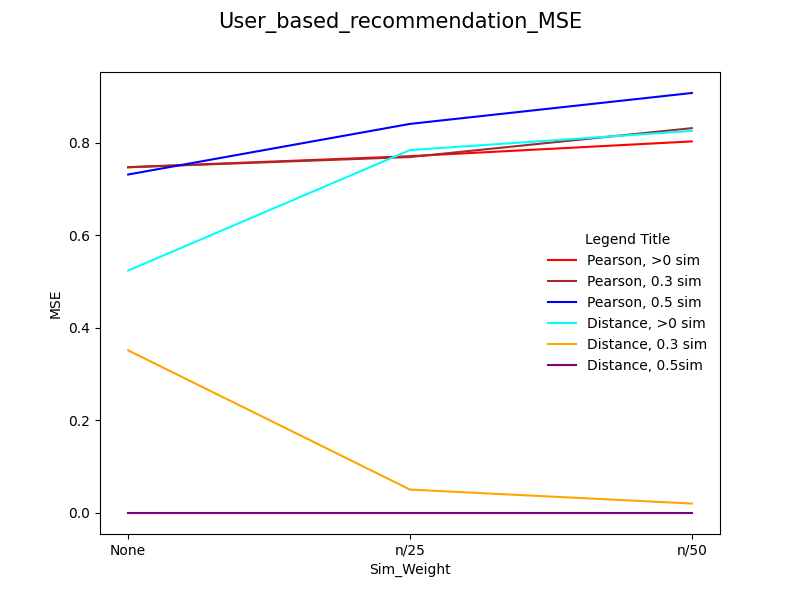
\includegraphics[width=4.5in]{User_based_MSE.png}
        \caption{User-based Recommendation, y-axis: MSE, x-axis: simWtg (none, n/25, n/50)}
        \Description{MSE measured for user-based}
    \end{figure}  
    \begin{figure}[h!]
        \centering
        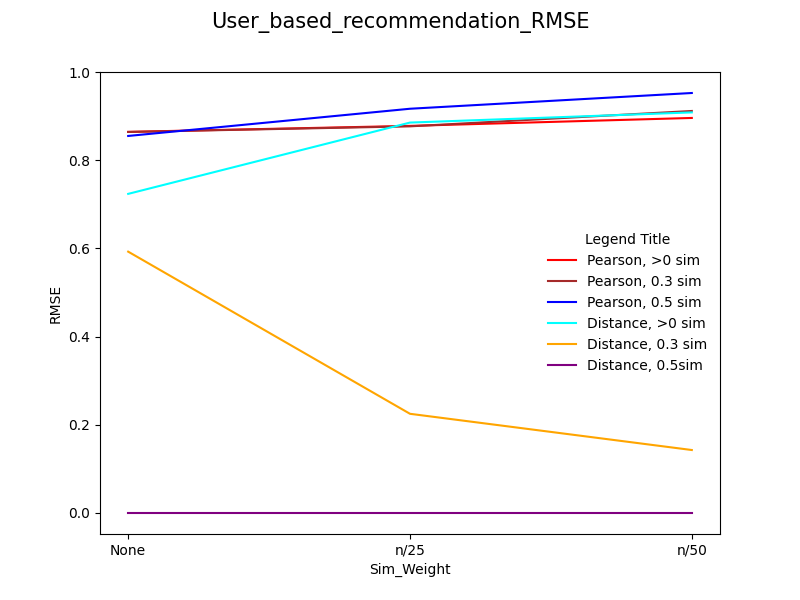
\includegraphics[width=4.5in]{User_based_RMSE.png}
        \caption{User-based Recommendation, y-axis: RMSE, x-axis: simWtg (none, n/25, n/50)}
        \Description{RMSE measured for user-based}
    \end{figure}  
    \begin{figure}[h!]    
        \centering
        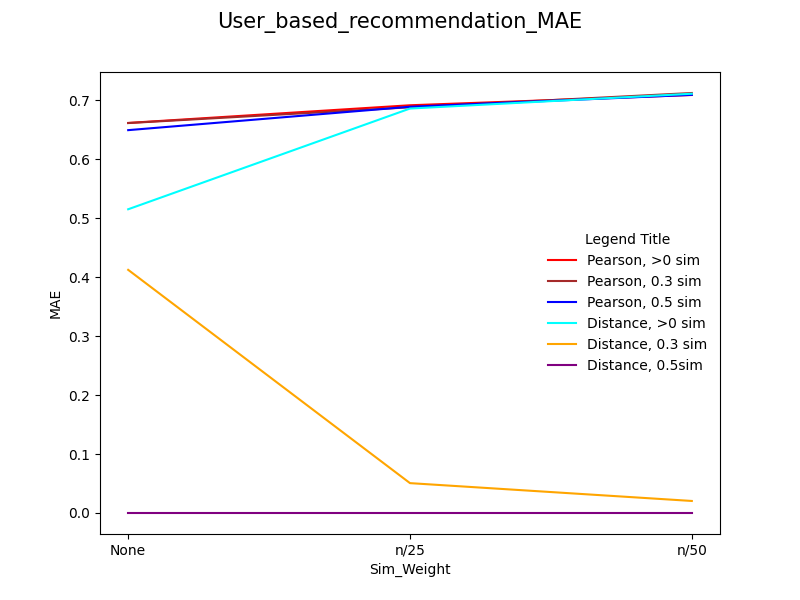
\includegraphics[width=4.5in]{User_based_MAE.png}
        \caption{User-based Recommendation, y-axis: MAE, x-axis: simWtg (none, n/25, n/50)}
        \Description{MAE measured for user-based}
    \end{figure}  
    \begin{figure}[h!]    
        \centering
        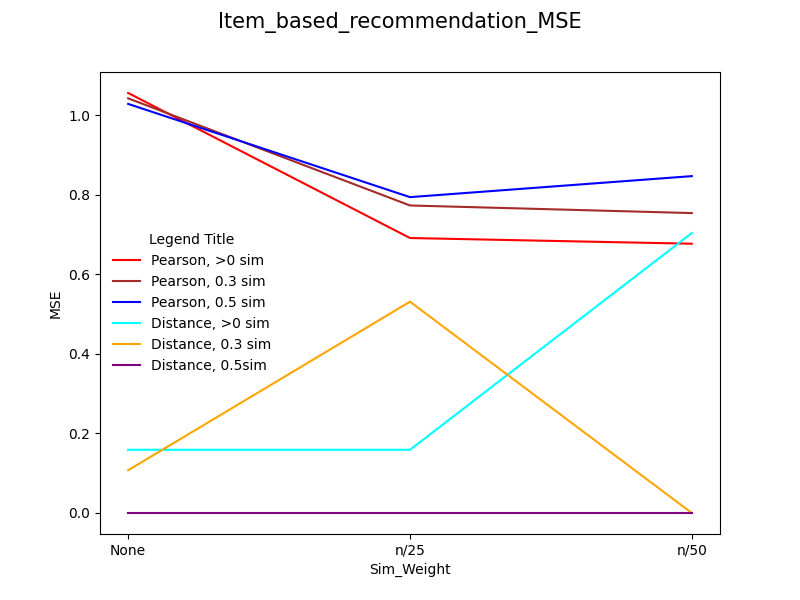
\includegraphics[width=4.5in]{Item_based_MSE.png}
        \caption{Item-based Recommendation, y-axis: MSE, x-axis: simWtg (none, n/25, n/50)}
        \Description{MAE measured for item-based}
    \end{figure}  
    \begin{figure}[h!]    
        \centering
        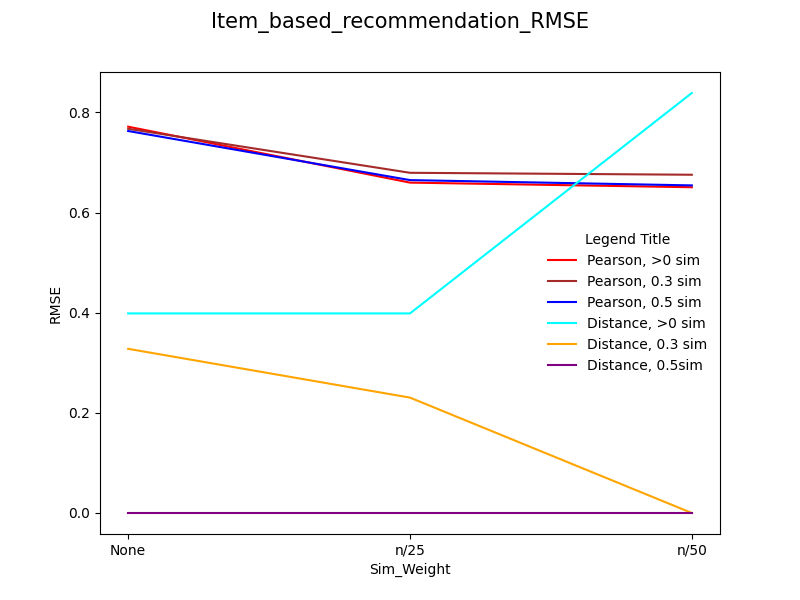
\includegraphics[width=4.5in]{Item_based_RMSE.png}
        \caption{Item-based Recommendation, y-axis: RMSE, x-axis: simWtg (none, n/25, n/50)}
        \Description{RMSE measured for item-based}
    \end{figure}  
    \begin{figure}[h!]    
        \centering
        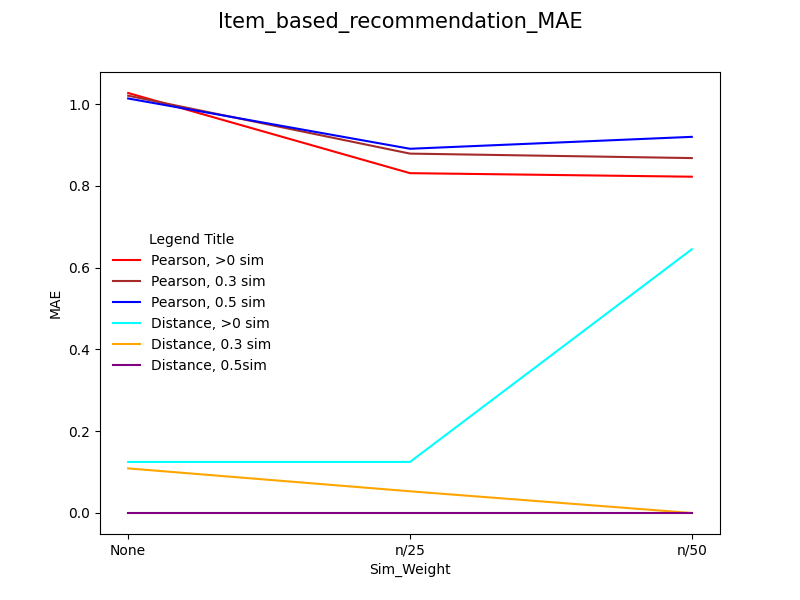
\includegraphics[width=4.5in]{Item_based_MAE.png}
        \caption{Item-based Recommendation, y-axis: MAE, x-axis: simWtg (none, n/25, n/50)}
        \Description{MAE measured for item-based}
    \end{figure}
    \begin{figure}[h!] 
    \centering
        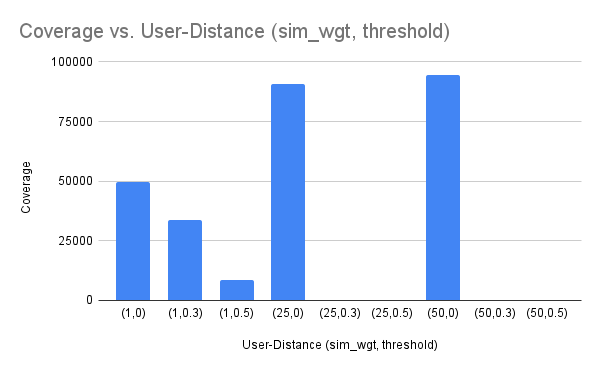
\includegraphics[width=4.5in]{Coverage vs. User-Distance (sim_wgt, threshold).png}
        \caption{Coverage vs. User-Distance}
        \Description{Coverage vs. User-Distance}
    \end{figure}
    \begin{figure}[h!] 
    \centering
        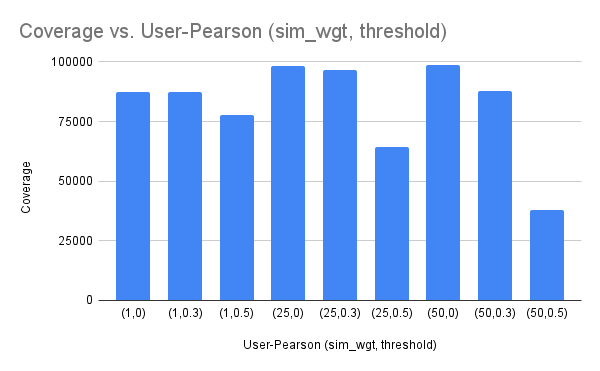
\includegraphics[width=4.5in]{Coverage vs. User-Pearson (sim_wgt, threshold).png}
        \caption{Coverage vs. User-Pearson}
        \Description{Coverage vs. User-Pearson}
    \end{figure}
    \begin{figure}[h!] 
    \centering
        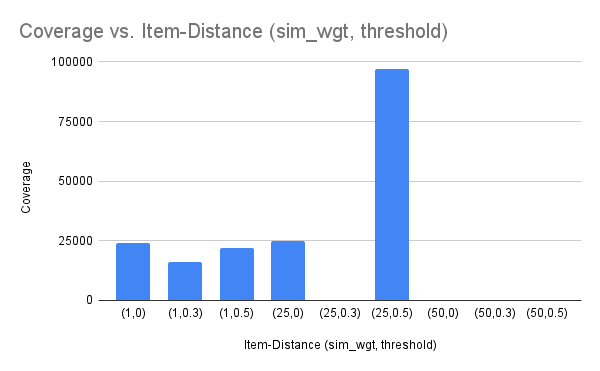
\includegraphics[width=4.5in]{Coverage vs. Item-Distance (sim_wgt, threshold).png}
        \caption{Coverage vs. Item-Distance}
        \Description{Coverage vs. Item-Distance}
    \end{figure}
    \begin{figure}[h!] 
    \centering
        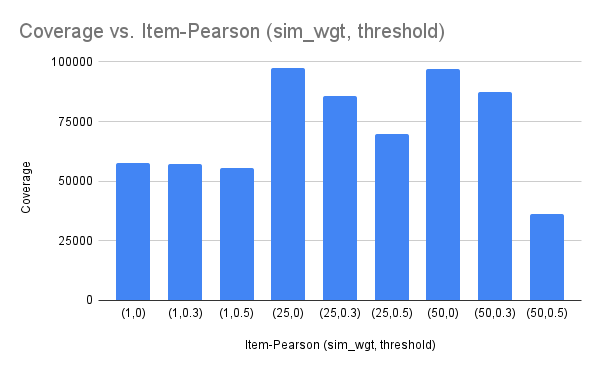
\includegraphics[width=4.5in]{Coverage vs. Item-Pearson (sim_wgt, threshold).png}
        \caption{Coverage vs. Item-Pearson}
        \Description{Coverage vs. Item-Pearson}
    \end{figure}

% \pagebreak
\newpage
\section{Discussion}
Based on our results, our original hypotheses were partially rejected. Pearson was able to provide a better coverage for both user and item-based algorithms. However, contrary to what we have thought, larger similarity and larger threshold did not produce the best result. For example, as we can see with the results of when similarity weight = 50 and similarity threshold = 0.5, it produced very little coverage. By our definition of a good recommender system, we would want high coverage. From this, we can conclude that higher similarity weighting and threshold should be relevant to the size of the dataset. In our case, applying a high similarity weighting and threshold made our similar users and items decrease tremendously, to the point where no accurate prediction can be generated due to the lack of similarity. \\
Additionally, we conducted a t-test by choosing a case where similarity weight was 25 and threshold was 0. This test helped us determine if there is a statistically significant difference between the means of our selected groups of data. We calculated a t-statistic and a p-value which allows us to compare MSE results(whether the means are equal) for three of our critics test cases. The results obtained are shown in the table below:
\begin{figure}[h!] 
    \centering
        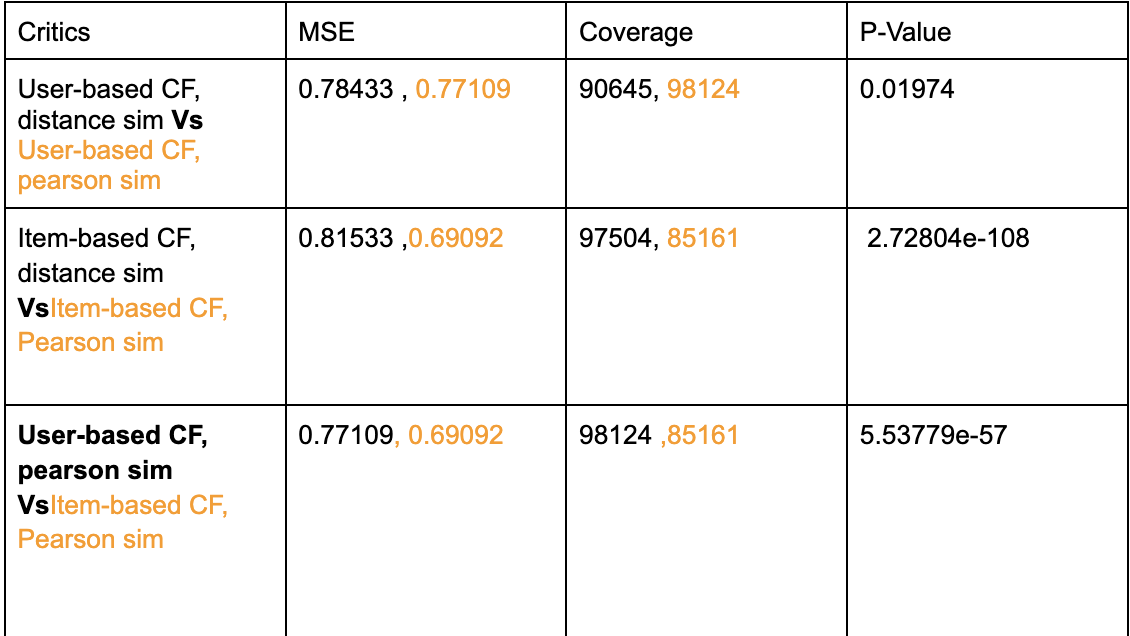
\includegraphics[width=4.5in]{t-test.png}
        \caption{T-test results}
        \Description{T-test results}
\end{figure}
\newline
After comparing the cases seen in figure 11, all of the comparisons reject the null hypothesis which states that the means are equal because the p-values were all lower than our chosen alpha value of 0.05.

Pearson correlation provides superior coverage and lower accuracy than Euclidean distance, while Euclidean distance provides higher accuracy at the expense of coverage. Because we consider higher coverage to be a more important metric, Pearson in that case fulfills the requirement better.
 
\section{Conclusion}
Our case study demonstrates that the user-based recommender system implemented with Pearson correlation, similarity weighting of n/25, and a threshold of 0 produces the best result overall. However, despite the general trend, there are some exceptions where the test cases of user-based Pearson and item-based Pearson did not produce conclusive results since there are minuscule differences in terms of accuracy and coverage between the two methods.
Therefore, in our future research, we would like to conduct tests with different ranges of datasets to conclusively determine which recommender algorithm performs better. For example, in our case where we defined our best recommender system as the one that provides the best coverage, which follows that the lower the threshold, the better the coverage. In this case, would our definition of a good recommender system offer the "best" recommender system? For further analysis, we can identify a threshold of coverage, so that once it reaches a good point of coverage, accuracy plays a more important weight on identifying the best recommender system. As we tested our datasets on different threshold values, coverage decreases dramatically as the threshold value increased. However, as our algorithms are applied to much larger datasets, it would not be practical to compute predictions using the ratings of all users. Therefore, the bigger concern lies between recognising what is more important for an effective recommender system: high coverage or higher accuracy. To strengthen our research, we plan to perform a more detailed analysis on a variety of thresholds in the future 

\section{Acknowledgments}

We are grateful to our CSC 381 professor Dr. Carlos Seminario who personally worked with us to help us navigate through the challenges in the project. 

\begin{thebibliography}{widest entry}
 \bibitem{her99} Jonathan L. Herlocker, Joseph A. Konstan, Al Borchers, John Riedl,  \emph{An Algorithmic Framework for Performing Collaborative Filtering}, 1999
 \bibitem{bad} Badrul Sarwar, George Karypis, Jospeph Konstan, and John Riedl, \emph{Item-Based Collaborative Filtering Recommendation Algorithms}, 2001
 \bibitem{car} Carlos Seminario, \emph{Moodle Slides}, 2022

\end{thebibliography}


\newpage

%%
%% The next two lines define the bibliography style to be used, and
%% the bibliography file.
%\bibliographystyle{ACM-Reference-Format}
%\bibliography{sample-base}









\end{document}
\endinput
%%
%% End of file `sample-manuscript.tex'.
